\chapter{Introducing directionality with diffusion tensors}
\label{chap:dti}

In this chapter, we focus on how to transfer information from
diffusion tensor imaging (DTI) data into our finite element
methods. To do so, we will need to overcome several practical
challenges. In particular, the DTI data uses a different coordinate
system than the mesh, and is stored at a different resolution; DTI
data can also display sharp transitions that will need to be
addressed. To overcome these challenges, we will use sub-sampling, and
smoothing, techniques in addition to co-registering DTI data with
several of the images we have already used in the construction of our
mesh.

Concretely, we will
\begin{itemize}
\item
  process the diffusion tensor images to extract mean diffusivity and
  fractional anisotropy data;
\item
  map the DTI tensor data into a finite element representation created from
  the T1-weighted images.
\end{itemize}

\section{Extracting mean diffusivity and fractional anisotropy}

\subsection{Extracting and converting DTI data}
\label{sec:chp-dti:extract-and-convert}

The DTI data must first be extracted from a DICOM dataset. We used
DicomBrowser to extract a DTI series from the book data set in
Chapter~\ref{sec:chp2:tools:viewers}; the resulting files are
available in \emp{dicom/ernie/DTI}. Our next task is to convert the
extracted DTI images to a single volume image and to produce
supplementary information files, about the DTI image data, for
downstream postprocessing.  Various open source tools are available
for the processing of DTI data \cite{soares2013hitchhiker}. Here, we
continue to use \freesurfer{} and its associated command-line tools
and in particular we launch the command \emp{mri\_convert}:
\terminal{\$ cd dicom/ernie/DTI \\
\$ mri\_convert IM\_0001 dti.mgz
}

This process, when successful, creates three files: \emp{dti.mgz},
\emp{dti.bvals}, and \emp{dti.voxel\_space.bvec}.  The last two, plain
text, files contain information regarding the "b-values" and
"b-vectors" associated with the DTI data. These values and vectors
measure the degree of the diffusion weighting applied in the imaging
process (b-values) and in what direction (b-vectors). The various
slices in the imaging sequence are measured for the different b-values
and b-vectors selected for the initial imaging study (see
Figure~\ref{fig:chp5:DTIslices}).
\begin{figure}	
\begin{center}
  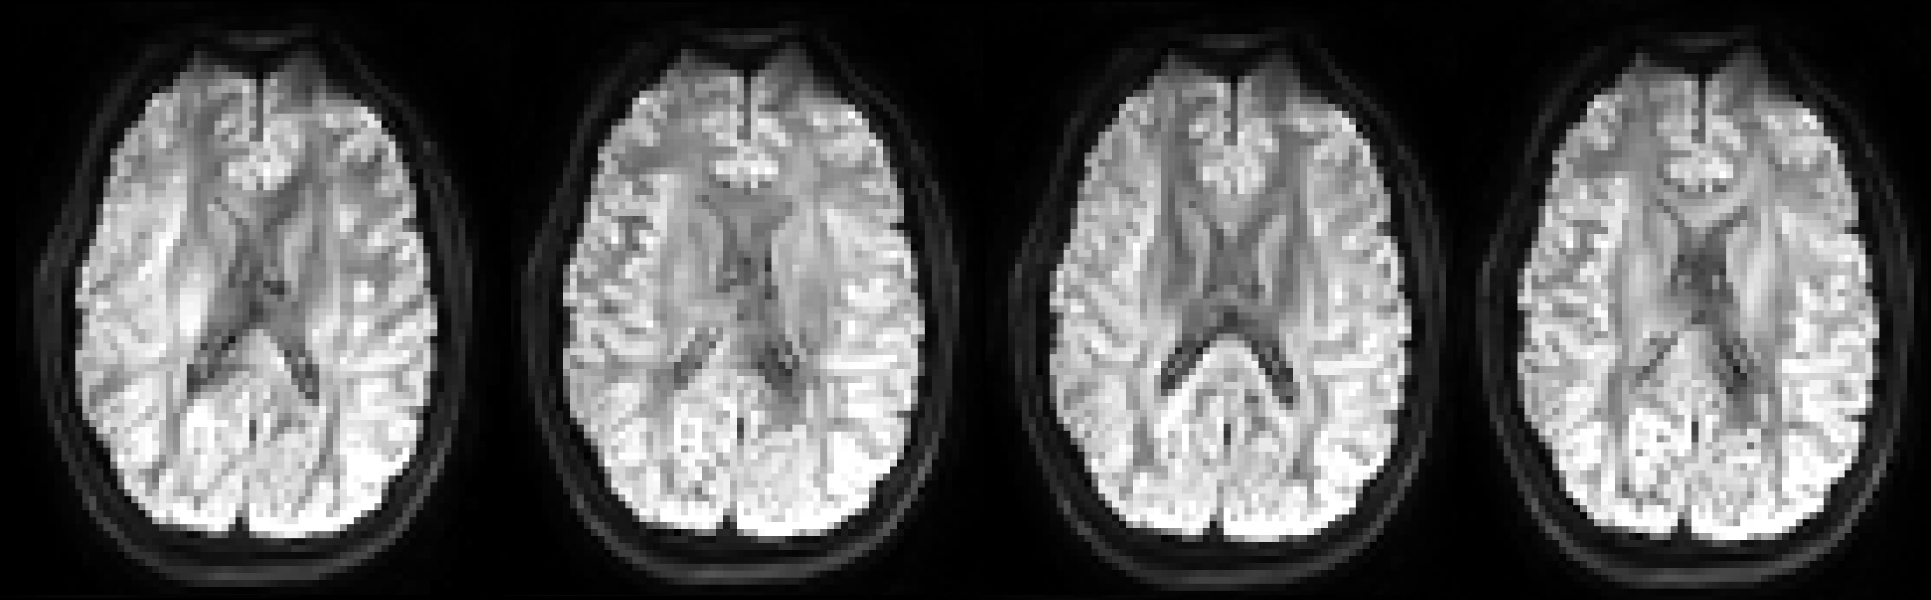
\includegraphics[width=0.95\textwidth]{./chapters/chp5/FIG/dwi.png}
\end{center}
\caption{Axial DTI slices measured with different b-vectors. The
  resolution in the DT image is typically lower (here, 96x96x50)
  compared to in the T1 images.}
\label{fig:chp5:DTIslices}
\end{figure}

\subsection{DTI reconstruction with \freesurfer}
\label{sec:chp-dti:freesurfer-dtrecon}

Next, we aim to reconstruct comprehensive DTI data from the volume,
b-value, and b-vector files using the \freesurfer{} command
\emp{dt\_recon}. The command takes an input volume (following
\emp{-{}-i}), b-vector and b-values files (following \emp{-{}-b}), an
output directory \emp{-{}-o} and the \emp{recon-all} subject id
\emp{-{}-s}. Within our book data directory \emp{dicom/ernie/DTI}, we
can launch the following commands:
\terminal{\$ export SUBJECTS\_DIR=my-freesurfer-dir \\
  \$ dt\_recon -{}-i dti.mgz -{}-b dti.bvals dti.voxel\_space.bvecs -{}-s ernie -{}-o \$SUBJECTS\_DIR/ernie/dti}
\noindent with \emp{my-freesurfer-dir} replaced by the FreeSurfer subjects
directory (e.g. \emp{freesurfer/} from the book data set).

This command produces multiple output files; including
\emp{tensor.nii.gz}, \emp{register.dat} and \emp{register.lta}. The
registration in \emp{dt\_recon} uses the registration command
\emp{bbregister} to register the DTI
data~\cite{freesurfer-wiki}. Files with the suffix .nii are in the
NIfTI format. Of these, \emp{tensor.nii.gz} is the spatially-varying
diffusion tensor. Further, an eigendecomposition of this tensor in
terms of spatially-varying eigenvalues $\lambda_1, \lambda_2,
\lambda_3$ and eigenvectors $v_1, v_2, v_3$ are given in the files
\emp{eigvals.nii.gz}, and \emp{eigvec1.nii.gz},\emp{eigvec2.nii.gz},
and \emp{eigvec3.nii.gz}.


\subsection{Mean diffusivity and fractional anisotropy}

In addition, \emp{dt\_recon} produces the NIfTI files
\emp{adc.nii.gz} and \emp{fa.nii.gz} for the mean (or apparent)
diffusivity (MD) and fractional anisotropy (FA), respectively. 
The mean diffusivity is given by 
\begin{equation}
  \rm{MD} = \frac{1}{3}(\lambda_1 + \lambda_2 + \lambda_3),   
\end{equation}
where $\{\lambda_i\}_i$ are the eigenvalues of the diffusion tensor.
and is associated to the volume file \emp{adc.nii.gz}. The fractional
anisotropy is defined~\cite{kindlmann2007geodesic} by
\begin{equation}
\rm{FA}^2 = \frac{1}{2} \frac{\lambda_1-\lambda_2)^2 
+ (\lambda_2 - \lambda_3)^2 + (\lambda_3 - \lambda_1)^2}{\lambda_1^2 
+ \lambda_2^2 + \lambda_3^2} 
%= \sqrt{3/2 \frac{ \sqrt{(dev(D_{ij}), dev(D_{ij}))}}{\sqrt{(D_{ij},D_{ij})}}}.
\end{equation}

\begin{figure}	
  \begin{center}
    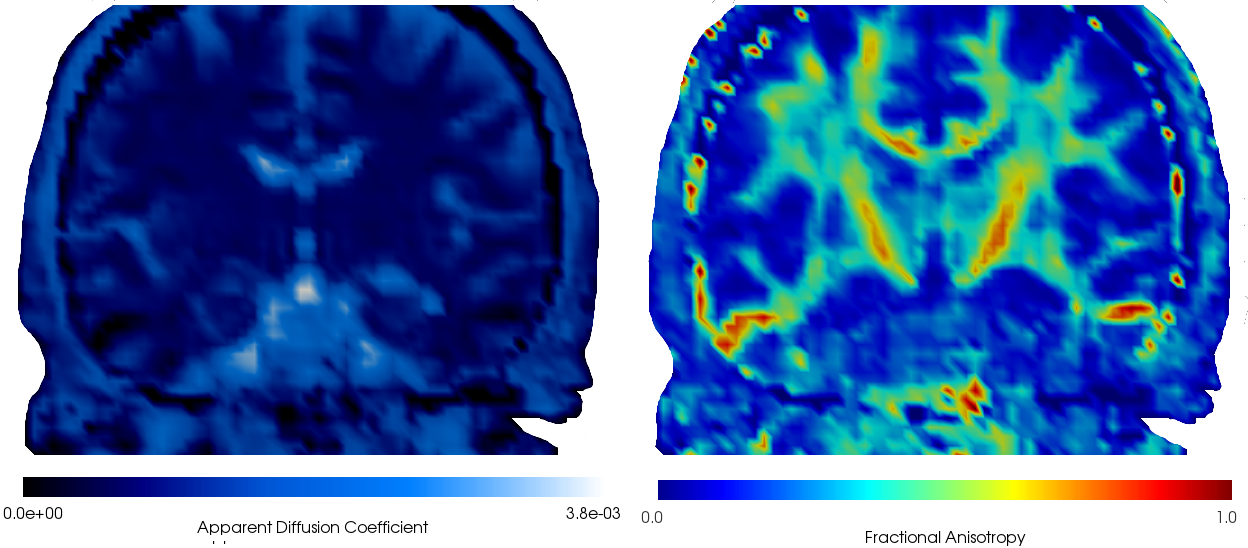
\includegraphics[width=0.95\textwidth]{./chapters/chp5/FIG/paraview_adcfa.png}
  \end{center}
  \caption{Mean diffusivity (left) and fractional anisotropy (right) as shown in \emp{Paraview}.}
  \label{fig:chp5:DTIfa}
\end{figure}
NIfTI files can be viewed in ParaView. You may first need to enable
the NIfTI viewer plugin by selecting the Paraview menu option
\button{Tools--Manage Plugins}, select the plugin option labeled
\button{AnalyzeNifTIIO} and then click \button{Load Selected}.  You
can then open and view (zipped) .nii files as you would any other
file in Paraview. Try opening the files \emp{adc.nii.gz} and
\emp{fa.nii.gz}; the results should look something like
Figure~\ref{fig:chp5:DTIfa}.

In general, the average FA is around 0.5 and changes by around 2\%
during day/night~\cite{voldsbekk2020evidence}; anisotropy decrease
with age, e.g.~around 14\% from 30 to 80
years~\cite{kochunov2011fractional}; and anisotropy can change up to
50\% in certain areas in an Alzheimer's disease patient compared with
healthy subjects~\cite{naggara2006diffusion}. In the \emp{ernie} data,
c.f.~Figure~\ref{fig:chp5:DTIfa}, the median white-matter FA value is
0.3, with a minimum of 0.009, and a maximum of 0.9998.
%% In closing, we
%% note that Eigenvalues computed by {\freesurfer} are sometimes
%% negative; clearly, this is not a physical result and DTI data must be
%% checked before it can be safely used in mathematical models.  Data can
%% be checked by opening the files, which all have self-explanatory
%% names, for the complete tensor, the eigenvalues and the eigenvectors.

\section{A finite element representation of the diffusion tensor}

In this section, we aim to
\begin{itemize}
\item
  improve on the DTI data to yield a valid eigendecomposition;
\item
  map the DTI tensor into a finite element tensor function defined on
  a finite element mesh;
\item
  briefly discuss co-registration.
\end{itemize}

\subsection{Preprocessing the diffusion tensor data}

The DTI data can be quite rough compared to the T1 data and our
corresponding finite element meshes. Moreover, the signal can be
disturbed close to the CSF, which makes the data in certain areas of
the cortical grey matter and in the regions near the ventricle system
less reliable. Indeed, inspection of the eigenvalues of the DTI tensor
shows non-physiological (zero and/or negative) eigenvalues. To ensure
a physiologically (and mathematically) reasonable diffusion tensor, we
recommend preprocessing the diffusion tensor prior to numerical
simulation. In particular, we here present two scripts that
\begin{itemize}
\item
  check the DTI tensor data for non-physiological values;
\item
  replaces non-physiological by physiological values in the DTI tensor,
\end{itemize}
respectively.

\subsubsection*{Creating brain masks}

To aid in this process, we will use \freesurfer{} to create so-called
masks of the brain i.e.~filters where voxels (significantly) outside
the brain are set to zero. Using our white matter parcellation data
(included in \emp{freesurfer/ernie/mri/wmparc.mgz}), brain masks can be
  created as follows:
\terminal{\$ mri\_binarize --i wmparc.mgz --gm --dilate 2 --o mask.mgz}
\noindent The \emp{dilate} determine how much the mask should be
extended outside the brain surface provided by
\emp{wmparc.mgz}. Examples of such masks are shown in
Fig.~\ref{fig:chp5:masks}.
\begin{figure}	
\begin{center}
  
\includegraphics[trim=400 130 500 150,clip,width=0.49\textwidth]{./chapters/chp5/FIG/mask0.png}
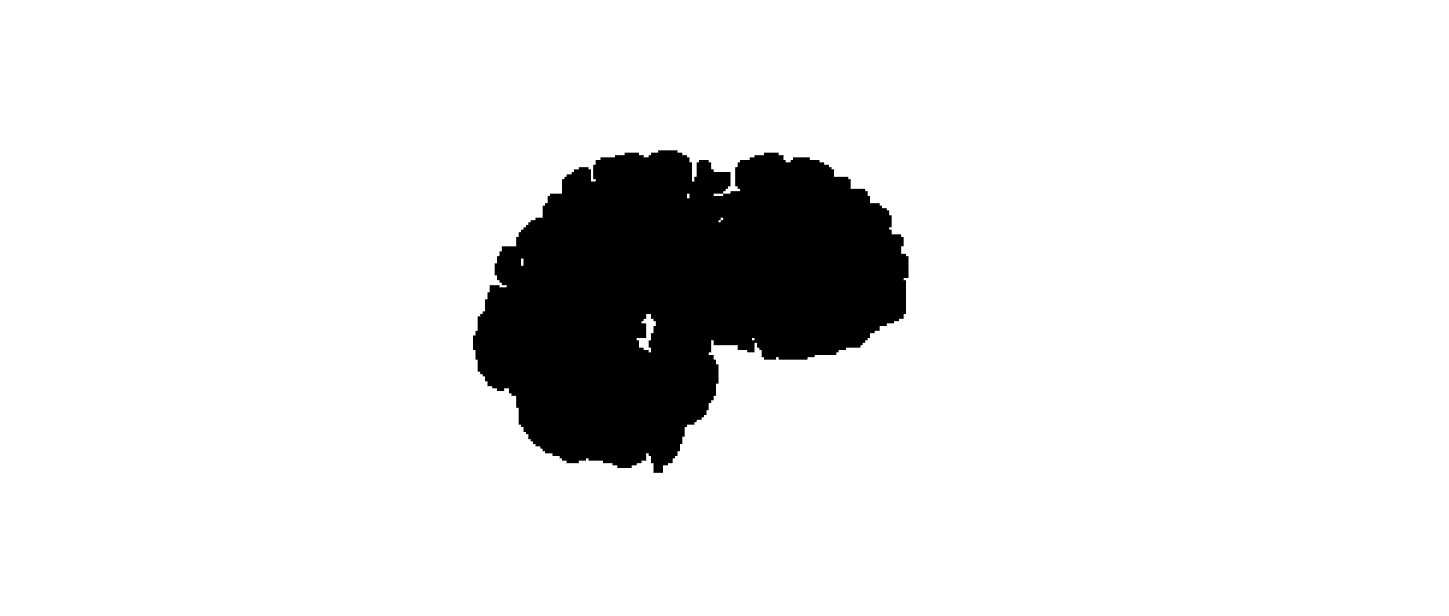
\includegraphics[trim=400 130 500 150,clip,width=0.49\textwidth]{./chapters/chp5/FIG/mask1.png} \\
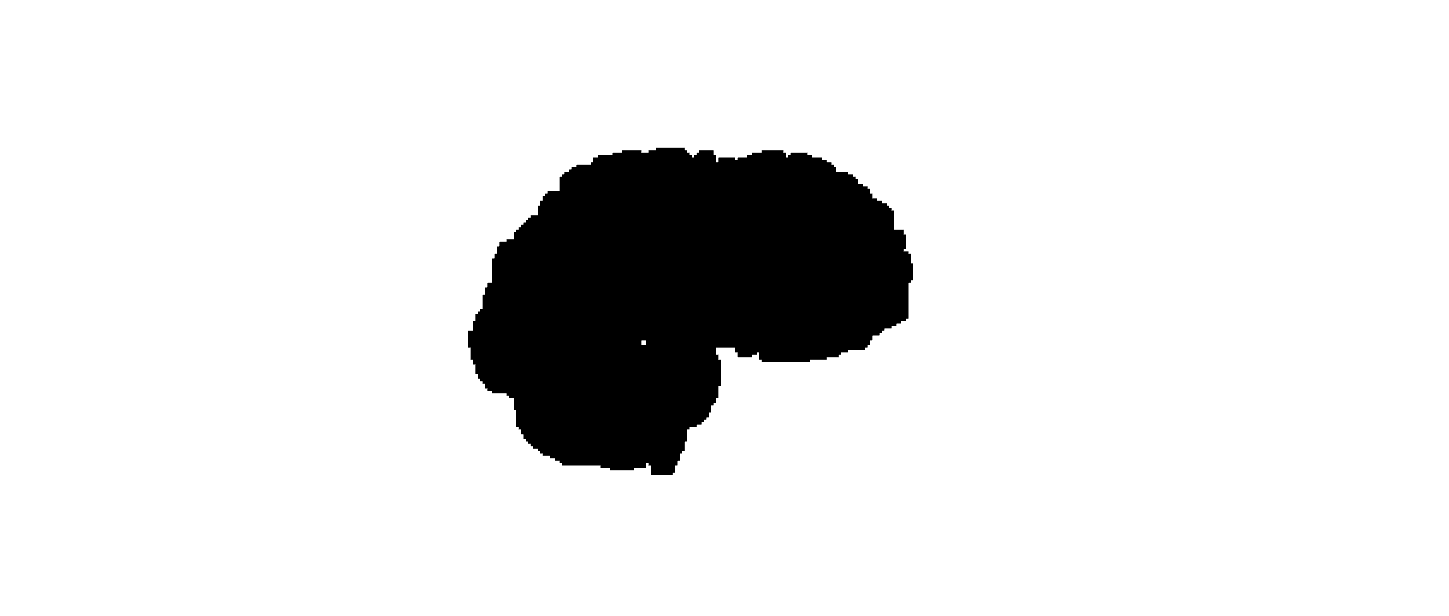
\includegraphics[trim=400 130 500 150,clip,width=0.49\textwidth]{./chapters/chp5/FIG/mask2.png}
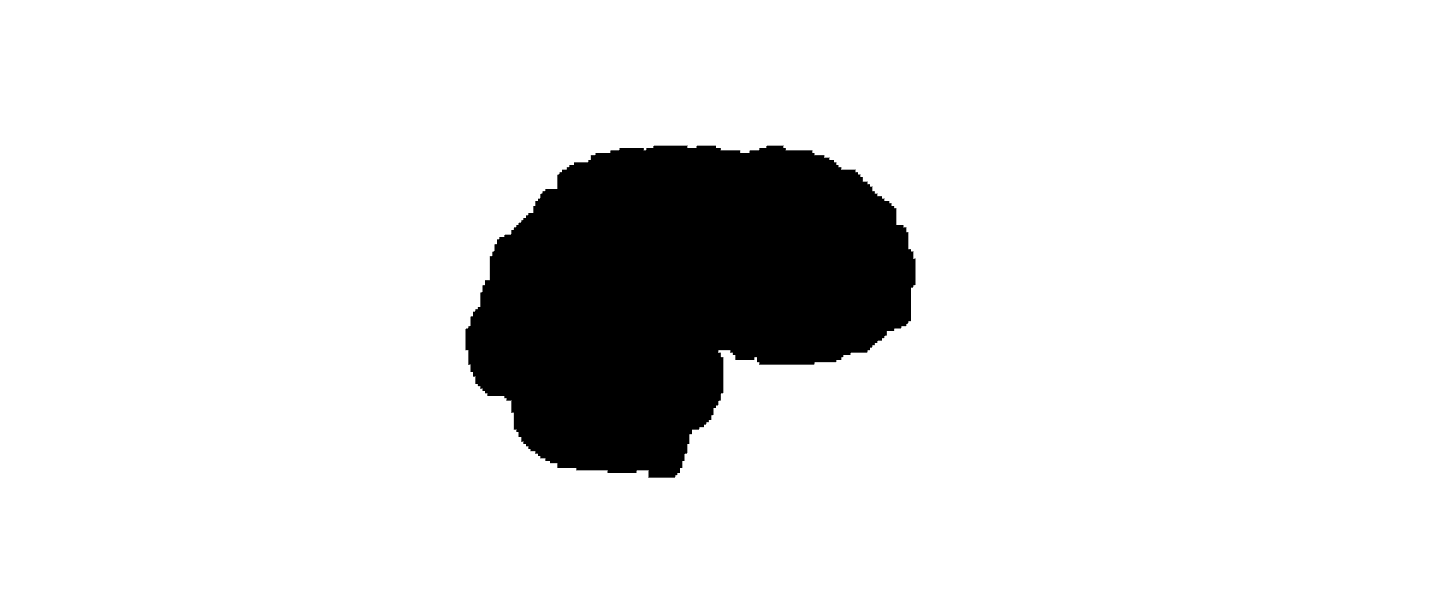
\includegraphics[trim=400 130 500 150,clip,width=0.49\textwidth]{./chapters/chp5/FIG/mask3.png}
\end{center}
\caption{
  Brain masks created using \emp{mri\_binarize} with \emp{dilate} ranging from 0 to 3.
}
\label{fig:chp5:masks}
\end{figure}

\subsubsection*{Examining the DTI data values}

We can work with the DT image data in a very similar manner as we did
for the parcellation (image) data in
Chapter~\ref{sec:chp4:mapping_parcellation}. We will again use NiBabel
to load the image data, use the \emp{vox2ras} functions for mapping
between the different image coordinate systems (DTI voxel space and T1
voxel space), and process the data as NumPy arrays. The complete
script can be run as:
\terminal{\$ cd mri2fem/chp5\\
\$ python3 check\_dti.py -{}-dti tensor.nii.gz -{}-mask mask.mgz}

We import the key packages:
\newpythonsnippet{chp5}{check_dti.py}{1}{6}

\noindent We define the function \emp{check\_dti\_data} that takes the DTI
tensor and mask files as input: 
\newpythonsnippet{chp5}{check_dti.py}{8}{20}

\noindent Now, the important coordinate transformations can be handled as follows:
\newpythonsnippet{chp5}{check_dti.py}{21}{30}

\noindent Before computing eigenvalues:
\newpythonsnippet{chp5}{check_dti.py}{33}{37}
and computing the fractional anisotropy and checking the validity of each voxel value:
\newpythonsnippet{chp5}{check_dti.py}{46}{58}

\subsubsection*{Improving the DTI values by extrapolation}
\mer{Lars: Could you check that the code examples run!! Something is amiss here.}

In the case that there are numerous invalid voxels, we can try
improving on the DTI data by extrapolating the adjacent valid
voxels. The complete
script can be run as:
\terminal{\$ cd mri2fem/chp5\\
\$ python3 clean\_dti\_data.py -{}-dti tensor.nii.gz -{}-mask mask.mgz -{}-out\_nii tensor-clean.nii}
\noindent and the main functionality reads as:
\newpythonsnippet{chp5}{clean_dti_data.py}{26}{48}

The function \pythoninline{find_valid_adjacent_tensor} will search for a valid
tensor in the adjacent voxel, and iteratively increase the search if
no valid tensor is found. We define a valid tensor
based on a non-zero sum of the MD. If there are multiple valid tensors within
the search, then the tensor with the MD closest to the median of non-zeros MD is
chosen.
\newpythonsnippet{chp5}{clean_dti_data.py}{7}{24}

\subsection{Representing the DTI tensor in \fenics{}}
\label{chp5:sec:loading-dti-tensor}

We are now ready to map our preprocessed DTI image (now in T1 voxel
space) onto a FEniCS mesh. We assume that we have a \emp{mesh}
available (for instance \emp{ernie-brain-32.h5} from
Chapter~\ref{chp4:meshio-converting}), that we have loaded the clean DTI
image and data in \emp{dti\_image} and \emp{dti\_data} and that that
we have the \emp{ras2vox} transform associated with this image:
\newpythonsnippet{chp5}{dti_data_to_mesh.py}{49}{51}

To represent the diffusion tensor in FEniCS, we create a FEniCS
\emp{Function} over a \emp{TensorFunctionSpace} of (discontinuous)
piecewise constant polynomial fields (\emp{"DG", 0}): 
\newpythonsnippet{chp5}{dti_data_to_mesh.py}{53}{55}

We could now extract the cell midpoints as we have done before, but we
can also extract the coordinates of the degrees of freedom of the
function space and convert these to voxel indices:
\newpythonsnippet{chp5}{dti_data_to_mesh.py}{57}{68}

We can now reshape the DTI data into a cell-wise structure,
\newpythonsnippet{chp5}{dti_data_to_mesh.py}{70}{72}
\noindent assign it to the FEniCS tensor field \pythoninline{D},
\newpythonsnippet{chp5}{dti_data_to_mesh.py}{78}{79}
and save it with the mesh: 
\newpythonsnippet{chp5}{dti_data_to_mesh.py}{87}{90}
The resulting fiber directions can be inspected in Figure~\ref{fig:chp5:freesurfer-parc}.
\begin{figure}	
  \begin{center}
  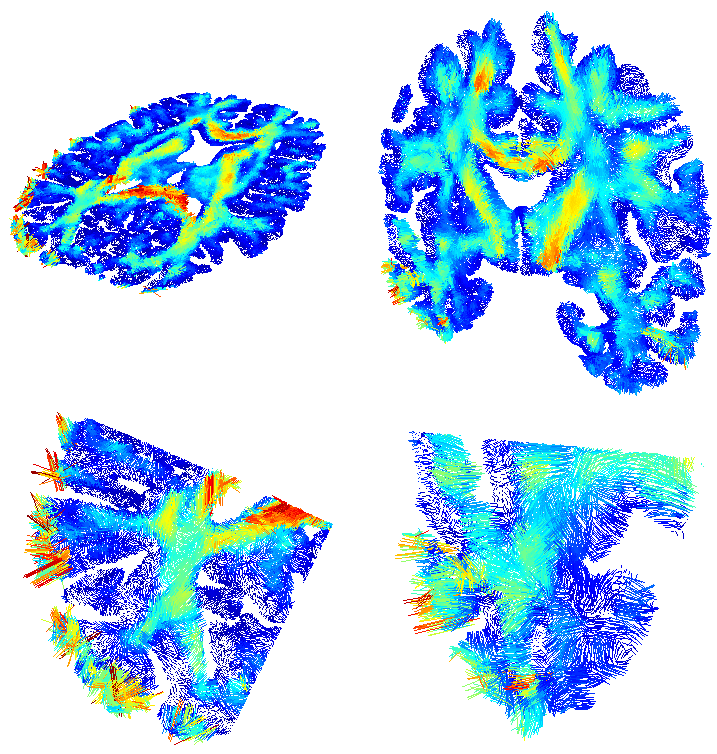
\includegraphics[width=0.8\textwidth]{./chapters/chp5/FIG/fiber-fa-2.png}
  \end{center}
\caption{Upper panels show fiber directions (DTI eigenvectors) colored
  by the fractional anisotropy in the axial and coronal plane. The
  lower panels show a zoom focusing on the boundary between grey
  matter and the CSF.}
\label{fig:chp5:freesurfer-parc} 
\end{figure}




%% We have added the function \pythoninline{adjusting_mean_diffusivity}, which allows the user to specify the minimum and maximum values inside a subdomain. The subdomains are determined by the tags set in {\svmtk} and any updates to the subdomains, like parcellations, that we mentioned in chapter \ref{sec:chp4:addparcellations}.

%% \pythonsnippet{chp5}{dti_data_to_mesh.py}{10}{31}

%% The function will first compute the MD, and then go through the input of limits. The limits is an Nx3 array, containing the subdomain label/tag, the lower and the upper MD limits. Setting either of the limits to zero will set the limits at infinity or minus infinity. This effectively cause the mask to be empty and thus having no effect on the data. 

%% We first sett the MD to 1 for all values outside the lower and upper limits. Then, the function will multiple the tensor with the appropriate limits. This can also be used to normalize the tensor based on the MD by setting both upper and lower limit equal to 1. In order to utilize this property, we can add Nx3 array to the function call like.
%% \begin{python}
%% dti_data_to_mesh("ernie.h5", "clean-dti-data.mgz","ernie.h5",[1,5.0e-5,1.0e-3])
%% \end{python}

%% We save the DTI tensor function together with the in a .h5 file, and we will use this tensor in the next chapter.
%% \pythonsnippet{chp5}{dti_data_to_mesh.py}{83}{95} 


\subsection{A note on co-registering DTI and T1 data}
\label{sec:chp-dti:freesurfer-coord}

As we have seen {\freesurfer} uses several different coordinate
systems for labeling the position of data in its various output
files. Thus, to combine data from different modalities, we need to
extract information about the different coordinate systems and be able
to map between these. This process is known as co-registration. We
have used NiBabel functionality to handle this process, but
include some additional information on co-registration here for context.

%% We aim to use our DTI data alongside the meshes and parcellations
%% created from the T1 images in the previous chapters. In order to do
%% so, we first need to consider co-registration -- a process that allows
%% us to transfer data between different {\freesurfer} output files. In
%% particular, {\freesurfer} uses several different coordinate systems
%% for labelling the position of data in its various output files, and
%% thus to combine data from different modalities, we need to be able to
%% map between the different coordinate systems. 

In short, let $x_1 = (x_1, y_1, z_1)$ and $x_2 = (x_2, y_2, z_2)$ represent the
same physiological point in $\R^3$ but represented with respect to two
different coordinate systems (bases). Then, there is an affine
transformation such that
\begin{equation} 
x_2 = A\, x_1 + b,
\end{equation}
for $A \in R^{3 \times 3}$ and $b \in \R^3$. Determining the
transformation matrix $A$ and vector $b$ for a pair of files is the
co-registration.

The key step in co-registration is to ascertain the type of coordinate system used 
for the files related to the T1 images, and those related to the DTI images. To 
to this end, we use the \emp{mri\_info} command. We begin by inspecting the T1 files:
\terminal{\$ cd \$SUBJECTS\_DIR/ernie/mri \\
\$ mri\_info orig.mgz -{}-orientation \\
LIA}
\noindent The output \emp{LIA}, above, means that the T1 image files
were generated with respect to the `Left Inferior Anterior' coordinate
system (see~\cite{freesurfer-wiki} for details).

To determine the DTI data coordinate system, we do the same for the
generated tensor NIfTI file:
\terminal{\$ cd \$SUBJECTS\_DIR/ernie/dti \\
\$ mri\_info tensor.nii.mgz -{}-orientation \\
LPS}
Let's break down the result of \emp{LPS}; the first letter determines the 
positive direction in the sagittal plane and can be either (L)eft or (R)ight; 
the second letter determines the positive direction in the coronal plane and 
can be either (P)osterior or (A)nterior; the third letter determines the positive 
direction in the axial plane and can be either (I)nferior and (S)uperior. 
Thus, the coordinate systems \emph{LIA} and \emph{LPS} differ by a choice of 
positive direction in the second and third axes. To co-register these images, 
then, we can swap the orientation of these two axes.

%% To close this section we provide an example of a transformation that could be 
%% used to convert imaging data from the so-called Voxelspace coordinate system 
%% to the so-called SurfaceRAS coordinate system; this is for illustration purposes 
%% to make the conversation concrete.  In a terminal type the following command 
%% \terminal{\smpprmpt{\emp{mri\_info} orig.mgz -{}-vox2ras-tkr}}
%% \noindent You will see the following output in the terminal window
%% \terminal{\outprmpt{
%% \begin{tabular}{rrrr}
%%   -1.00000   & 0.00000  &  0.00000 & 128.00000 \\
%%    0.00000   & 0.00000  &  1.00000 &-128.00000 \\
%%    0.00000   &-1.00000  &  0.00000 & 128.00000 \\
%%    0.00000   & 0.00000  &  0.00000 &   1.00000
%% \end{tabular}}}
%% \noindent  The above output means that if we wanted to convert coordinates expressed 
%% in terms of Voxelspace coordinates, $x_V = (x_V,y_V,z_V)$, to coordinates expressed 
%% in SurfaceRAS coordinates, $x_R = (x_R,y_R,v_R)$, we would use the transformation 
%% matrix $A$ and vector $b$ given by   
%% \[
%% A=\left[\begin{array}{ccc} -1 & 0 & 0 \\
%%                            0 & 0 & 1 \\
%%                            0 & -1 & 0
%% \end{array} \right], \quad \mbox{and} \quad  
%% b=\left[\begin{array}{c} 128  \\
%%                         -128  \\
%%                          128 
%% \end{array} \right], 
%% \]
%% and that the voxel dimension, indicated by the bottom-right output, is 
%% $1.0\times 1.0 \times 1.0$.  That is
%% \[
%% x_R = \left[\begin{array}{ccc} -1 & 0 & 0 \\
%%                            0 & 0 & 1 \\
%%                            0 & -1 & 0
%% \end{array} \right]\,x_V + \left[\begin{array}{c} 128  \\
%%                         -128  \\
%%                          128 
%% \end{array} \right].
%% \]  



%\section{XX TBD}

%We can see in Figure (insert DTI figure) that the diffusion tensor is a spacial variable, and as such we can define it as a \emp{Function} in FEniCS. In order to do this, we must first decide what type of element we should use to represent the tensor. We often consider tensors as cell data, therefore the selection of P0 seems to fit with diffusion elements.   

%(i.e. P0,P1 elements etc)  


%A general problem is that tetrahedrons in our mesh does not fit with the voxel data as shown in Fig. ??. This can be solved by utilizing different interpolation methods, 




%It should be noted that interpolation of tensor does not preserve the tensor properties, like anisotropy, so different interpolation methods are often used instead. 

%An example of this is the interpolation between bifurcation of an axon bundle in the white matter, see Fig ?? . The Euclidean interpolation will create a new tensor by averaging based on 
%\begin{equation}
%\mathbf{C}_{EL}(t) = (1-t)\mathbf{A} + t\mathbf{B} .
%\end{equation} 
%The resulting tensor will have a lower fractional anisotropy. 


%Therefore, we will introduce Linear Invariant(LI) interpolation. 
 






%On this mesh we may define a FEniCS tensor field $D$. However, a main problem is that this tensor field will be expressed in 
%the coordinate system of the mesh based on the T1 data, while we have the tensor field in 
%terms of another coordinate system. Hence, we will fetch the coordinates from the mesh, $x_{T1}$ and transform them 
%to the DTI based corresponding coordinates as $x_{T1} = A x_{DTI} + b$.  
%Then we may express $D(x_{DTI})$ which is simply \pythoninline{data} can be expressed in 
%terms of $D(x_{DTI}) = D(A^{-1}(x_{T1} - b))$. In other words, we extract the coordinates from the tensorfield made in FEniCS and
%transform them into the DTI coordinate system before we evaluate the DTI tensor. 
%
%Hence, we start by creating a  \pythoninline{TensorFunctionSpace} object. 
%The function \pythoninline{tabulate_dof_coordinates} provides us with the coordinates of each degree of freedom in this field. 
%The numbering is such that all dofs corresponding to the same cell is grouped together. For instance, the first 9 entries will contain identical 
%$\mathbb{R}^3$ vectors, namely the coordinates of the $3\times 3$ tensor of cell 0, before the next 9 entries which belongs to cell 1.      
%Hence, only every 9th coordinate will be unique. The following code re-shapes the coordinate into a suitable format. 
%\begin{python}
%DG0 = FunctionSpace(mesh, "DG",0)
%imap = DG0.dofmap().index_map()
%num_dofs_local =  imap.local_range()[1]-imap.local_range()[0]
%xyz = DG0.tabulate_dof_coordinates().reshape((num_dofs_local,-1))
%\end{python}
%Thus \emp{xyz} contains only one coordinate for each node, and we find the correspond voxel by applying the transformation matrix. 
%\begin{python}
%from nibabel.affines import apply_affine
%ijk = apply_affine(matrix,xyz).T
%i,j,k =np.rint(ijk).astype('int')  
%\end{python}
%It is encouraged to use \emp{paraview} to visually inspect that the transformation is suitable.   
%Below, we detail the various transformations. 
%
%First we look at the registration of DTI-images to T1-weighted images. This registration matrix can be found in the output folder of \emp{dt\_recon}, and if we provided the option \emp{-{}-lta} we might have two registration files. The default file is \emp{register.dat}, and as mentioned before, it contains the transformation matrix for registration in the Surface RAS coordinates. The optional registration file will have the filename provided with the option \emp{-{}-lta}, which we called \emp{registration.lta}. This registration file has the transformation matrix of the registration in voxelspace coordinates. Thus, the two registration files have different approach to obtain the complete transformation matrix.  
%The registration matrix can be obtained from the \emp{.dat} text file with the following function.
%\begin{python}
%def load_registration_dat(filename):
%    import numpy as np
%    with open(filename, 'r') as f:
%         matrix = np.array([i.strip(" \n").split(" ") 
%                  for i in f.readlines()[4:8]],dtype='float32')   
%    return matrix
%\end{python}      
%We can similarly obtain the registration matrix from \emp{.lta} text file using the function. 
%\begin{python}
%def load_registration_lta(filename}
%    import numpy as np
%    with open(filename, 'r') as f:
%         matrix = np.array([i.strip(" \n").split(" ") 
%                     for i in f.readlines()[8:12]],type='float32')   
%    return matrix
%\end{python}  
%\lmv{ no longer needed, as we use nibabel function resample\_from\_to. Thus we only need to read from the header vox2ras\_tkr, but I feel it should be here to illustrate the need for transformation. }  
% 
%We can now read the registration matrices into python with the provided function, so the next step is determine the complete transformation matrix. In our case, we want to obtain the transformation matrix from Surface RAS to DTI-voxelspace. There are two options, depending on which registration file is chosen, to construct the complete transformation matrix. Both options require that we obtain a transformation matrix from Surface-RAS to voxelspace, which is know as \emp{vox2ras\_tkr}.
%
%There are different methods to obtain the \emp{vox2ras\_tkr} affine matrix. The first method  is to obtain it from the header of a mgz-file.
%\begin{python}
%import nibabel as nb
%dti    = nb.load("orig.mgz")
%header = dti.header  
%vox2ras_tkr = header.get_vox2ras_tkr()
%\end{python}
%A more explicit implementation reads, 
%\begin{python}
%def get_vox2ras_tkr(t1):
%    ds = t1.header._structarr['pixdim'][1:4]
%    ns = t1.header._structarr['dim'][1:4] * ds / 2.0
%    v2rtkr = np.array([[-ds[0], 0, 0, ns[0]],
%                       [0, 0, ds[2], -ns[2]],
%                       [0, -ds[1], 0, ns[1]],
%                       [0, 0, 0, 1]], dtype=np.float32)
%    return v2rtkr
%    
%dti    = nb.load("tensor.nii.gz") 
%vox2ras_tkr = get_vox2ras_tkr(dti)
%\end{python}
%
%We are now ready to define the complete transformation matrix, form Surface-RAS to DTI-voxelspace. If we use \emp{registration.dat}, we need to invert the registration matrix in order to transform from Surface-RAS to DTI-Surface-RAS. Then we multiple with the inverted vox2ras\_tkr so that we can go from DTI-Surface-RAS to DTI-voxelspace.
%\begin{python}
%# dat file  contains is RAStkr(SurfaceRAS) to 
%# RAStkr  affine transformation matrix 
%regdat = load_registration_dat(filename)
%vox2ras = get_vox2ras_tkr(dti)
%matrix = np.linalg.inv(get_vox2ras_tkr(dti)).dot(regdat)   
%\end{python}
%If we use \emp{registration.lta}, we need to invert the transformation matrix from voxelspace and Surface-RAS. This is then multiplied with the inverted registration matrix so that we go from voxelspace to DTI-voxelspace.  
%\begin{python}      
%# lta file contains  vox2vox affine transformation matrix
%reglta = load_registration_lta(filename )
%vox2ras = orig.header.get_vox2ras_tkr()
%matrix = np.linalg.inv(vox2ras.dot(reglta)) 
%\end{python}
%
%It is worth mentioning that the transformation between coordinate system can have some problems with out of bounds voxels. In other words, the mesh can have some coordinates that corresponds to voxelspace that do not exists in the DTI-voxelspace. We can solve this by actively setting the coordinates to be within the bounds of the voxelspace. 
%\begin{python}
%i[data.shape[0]<=i]=data.shape[0]-1
%j[data.shape[1]<=j]=data.shape[1]-1
%k[data.shape[2]<=k]=data.shape[2]-1
%\end{python}





















